\documentclass[11pt,a4paper]{article}
\usepackage[utf8]{inputenc}
\usepackage[T1]{fontenc}
\usepackage[indonesian,provide=*]{babel}
\usepackage{lmodern}
\usepackage{microtype}
\usepackage{xcolor}
\usepackage{graphicx}
\usepackage{booktabs}
\usepackage{tabularx}
\usepackage{listings}
\usepackage{soul}
\usepackage{hyperref}
\usepackage{geometry}
\geometry{margin=2.5cm}

\definecolor{blueaccent}{HTML}{2783DE}
\definecolor{softblue}{HTML}{E5F2FC}
\definecolor{darktext}{HTML}{2C2C2B}
\definecolor{softgray}{HTML}{F3F4F6}
\sethlcolor{softgray}
\newcommand{\cmd}[1]{\hl{\texttt{#1}}}
\newcommand{\evidence}[2]{%
  \begin{figure}[htbp]\centering
  \includegraphics[width=\textwidth]{#1}
  \caption{#2}
  \end{figure}}

\lstset{basicstyle=\ttfamily\small, breaklines=true, frame=single,
  backgroundcolor=\color{softgray}, numbers=left, numberstyle=\tiny}

\hypersetup{colorlinks=true, linkcolor=blueaccent, urlcolor=blueaccent}

\title{Laporan Praktikum: Tutorial OpenMP\\{\large Pemrograman Paralel CPU dengan OpenMP dalam C}}
\author{Aufa Akmal Bunaya}
\date{4 Oktober 2026}

\begin{document}
\maketitle

\begin{abstract}
Laporan ini mendokumentasikan pengerjaan delapan latihan tutorial OpenMP beserta
mini-project perkalian matriks paralel. Seluruh program dikompilasi dengan GCC
13.3.0 memakai flag \cmd{-fopenmp} dan dijalankan secara nyata pada VM Linux
2 vCPU. Setiap latihan diverifikasi kebenarannya, modifikasi yang diminta
tutorial diimplementasikan dan diuji, serta pertanyaan investigasi dijawab
berdasarkan perilaku yang teramati. Latihan 8 mengukur speedup riil: pada
$n=10^8$ iterasi, 2 thread mencapai speedup 1,53 (efisiensi 0,76) dan 4 thread
mencapai speedup 1,68 (efisiensi 0,42, oversubscription pada 2 vCPU), dengan
selisih numerik serial--paralel $7{,}4\times10^{-13}$ di bawah toleransi
$10^{-8}$. Mini-project memverifikasi perkalian matriks $256\times256$:
versi paralel identik dengan serial (selisih $0{,}0$) dan mencapai speedup
2,00 pada 2 thread.
\end{abstract}

\tableofcontents
\newpage

\section{Lingkungan}
\label{sec:env}

\begin{tabularx}{\textwidth}{l>{\raggedright\arraybackslash}X}
\toprule
Komponen & Spesifikasi \\
\midrule
Mesin & VM \texttt{htch-runtime}, Ubuntu 24.04.5 LTS \\
CPU & AMD EPYC 9D25 126-Core, 2 vCPU tersedia \\
RAM & 7,7 GiB \\
Kompiler & GCC 13.3.0 (Ubuntu 13.3.0-6ubuntu2\textasciitilde24.04.1) \\
Flag & \cmd{-std=c11 -O2 -Wall -Wextra -fopenmp} (link: \cmd{-lm} bila memakai \texttt{math.h}) \\
Variabel & \cmd{OMP\_DYNAMIC=FALSE}; jumlah thread lewat \cmd{OMP\_NUM\_THREADS} \\
Jumlah thread uji & 1, 2, 4 (4 thread = oversubscription pada 2 vCPU, disengaja untuk diamati) \\
\bottomrule
\end{tabularx}

\evidence{shot_01_env.png}{Pemeriksaan lingkungan: versi GCC, jumlah vCPU, dan kompilasi pertama dengan \cmd{-fopenmp}.}

Seluruh program dibangun dengan satu perintah \cmd{make} memakai Makefile pada
bagian~\ref{sec:repro}. Tidak ada warning kompilasi pada 14 program.

\section{Exercise 1: Membuat tim thread}
\label{sec:ex1}
Berkas: \texttt{src/hello\_openmp.c}. Program mencetak ukuran tim sebelum dan
sesudah region paralel, dan setiap thread mencetak sapaan di dalam
\cmd{\#pragma omp critical}.

\evidence{shot_02_hello.png}{Dua eksekusi dengan 4 thread: urutan sapaan berbeda antar run, tetapi setiap thread tepat mencetak satu baris.}

Hasil investigasi:
\begin{enumerate}
\item Thread yang diminta vs aktual: \cmd{OMP\_NUM\_THREADS}=1, 2, 4 semuanya
dipenuhi persis (\texttt{team size} aktual = 1, 2, 4).
\item Urutan sapaan berubah antar run (tiga run 4-thread menghasilkan tiga
urutan berbeda) karena penjadwalan thread oleh OS tidak deterministik;
\cmd{critical} hanya menyerikan akses, tidak mengurutkan ID thread.
\item \texttt{printf} sebelum region dieksekusi tepat satu kali (oleh thread
awal), sedangkan di dalam region dieksekusi sekali per thread --- region
paralel dieksekusi penuh oleh setiap anggota tim.
\item \texttt{After} selalu muncul terakhir karena akhir region paralel
memiliki barrier implisit: thread awal baru melanjutkan setelah seluruh tim
tiba dan tersinkronisasi.
\end{enumerate}

\section{Exercise 2: Data shared dan private}
\label{sec:ex2}
Berkas: \texttt{src/data\_sharing.c}, memakai
\cmd{\#pragma omp parallel default(none) firstprivate(base) private(scratch)}.

\evidence{shot_03_sharing.png}{Setiap thread mendapat salinan privat \texttt{base}=10+t dan \texttt{scratch}=t\textsuperscript{2}; variabel asli di luar region tidak berubah.}

Hasil investigasi:
\begin{enumerate}
\item Perubahan \texttt{base} di dalam region tidak memengaruhi \texttt{base}
asli (\texttt{Outside: base=10}) karena \cmd{firstprivate} memberi tiap
thread \emph{salinan privat} yang diinisialisasi dengan nilai 10.
\item Mengganti \cmd{private(scratch)} menjadi \cmd{firstprivate(scratch)}
lalu mencetak nilainya sebelum assignment: setiap thread mengamati nilai
awal $-1$ (salinan dari nilai asli). Ini membuktikan \cmd{firstprivate}
menyalin nilai masuk, sedangkan \cmd{private} tidak.
\item Membaca \cmd{private(scratch)} sebelum assignment pertama tidak valid:
variabel privat tidak diinisialisasi, nilainya tak terdefinisi --- nilai
``kebetulan'' yang tercetak tidak boleh dianggap bermakna.
\item Menghapus \cmd{firstprivate(base)} dengan \cmd{default(none)} menggagalkan
kompilasi: \texttt{error: 'base' not specified} \texttt{in enclosing 'parallel'}.
Klausa \cmd{default(none)} memaksa setiap variabel yang dipakai di dalam
region dideklarasikan atribut data-sharing-nya secara eksplisit.
\end{enumerate}
Catatan: \cmd{firstprivate} pada sebuah \emph{pointer} hanya menyalin alamatnya;
seluruh thread tetap menunjuk memori yang sama. Kepemilikan memori harus
diputuskan terpisah dari kepemilikan variabel pointer.

\section{Exercise 3: Paralelisasi penjumlahan vektor}
\label{sec:ex3}
Berkas: \texttt{src/vector\_add.c} ($n=10^6$), memakai
\cmd{\#pragma omp parallel for default(none) shared(a,b,c,n) schedule(static)}.
Penyimpanan array bersifat shared; variabel loop \texttt{i} privat menurut
aturan worksharing-loop OpenMP.

\evidence{shot_04_vecadd.png}{Hasil identik (\texttt{errors=0}) pada 1, 2, dan 4 thread.}

Modifikasi yang diminta dan hasilnya:
\begin{enumerate}
\item Terverifikasi pada 1, 2, 4 thread: \texttt{c[0]=0.0 c[n-1]=2999997.0
errors=0}.
\item $c_i = \alpha a_i + b_i$ dengan $\alpha=2$
(\texttt{src/vector\_add\_alpha.c}, \texttt{alpha} ditambahkan ke klausa
\cmd{shared}): \texttt{c[n-1]=3999996.0 errors=0}, sesuai harapan $4i$.
\item Bentuk terpisah (\texttt{src/vector\_add\_separate.c}:
\cmd{\#pragma omp parallel} + \cmd{\#pragma omp for} di dalamnya)
menghasilkan nilai numerik yang sama persis. Bentuk ini berguna ketika
beberapa operasi worksharing memakai ulang tim yang sama.
\item Jika baris \cmd{omp for} dihapus dari struktur terpisah, \emph{setiap}
thread mengeksekusi seluruh loop: terjadi data race pada \texttt{c} karena
beberapa thread menulis lokasi memori yang sama tanpa sinkronisasi.
Penulisan konkuren yang ``kebetulan identik'' tetap merupakan data race ---
model memori tidak menjamin hasilnya.
\end{enumerate}
Pemeriksaan ketergantungan: loop seperti \texttt{a[i] = a[i-1] + b[i]}
memiliki dependensi antar iterasi yang berdekatan; menambah \cmd{parallel for}
tidak menghilangkan dependensi tersebut.

\section{Exercise 4: Akumulasi aman dengan reduction}
\label{sec:ex4}
Berkas: \texttt{src/sum\_methods.c} menjumlah $1\ldots10^6$
(ekspektasi $500000500000$) dengan tiga metode yang benar.

\evidence{shot_05_sum.png}{Ketiga metode menghasilkan nilai yang tepat pada 4 thread.}

Hasil investigasi:
\begin{enumerate}
\item Ketiga metode benar pada 1, 2, dan 4 thread (\texttt{exit=0}).
\item \texttt{sum\_reduction} tidak boleh sekaligus tercantum di
\cmd{shared(...)} pada direktif yang sama: klausa \cmd{reduction} sudah
memberi setiap partisipan akumulator privat yang digabungkan di akhir;
variabel yang sama tidak dapat berstatus shared dan reduction sekaligus.
\item Jumlah kuadrat $1\ldots1000$ dengan reduction
(\texttt{src/sum\_squares.c}): \texttt{expected=333833500 got=333833500 OK},
sesuai rumus $n(n+1)(2n+1)/6$.
\item Pengukuran waktu ketiga metode ($n=10^7$, 5 repetisi, 4 thread,
tanpa pencetakan di dalam timer):
\end{enumerate}

\begin{center}
\begin{tabular}{lrr}
\toprule
Metode & Waktu/run (s) & Relatif terhadap reduction \\
\midrule
\cmd{reduction} & 0,002970 & $1\times$ \\
\cmd{atomic update} & 0,230224 & $78\times$ \\
\cmd{critical} & 0,508649 & $171\times$ \\
\bottomrule
\end{tabular}
\end{center}

Reduction jauh lebih cepat karena tiap thread mengakumulasi secara lokal
tanpa sinkronisasi per iterasi dan hanya digabungkan sekali di akhir;
\cmd{atomic} dan \cmd{critical} menyerikan setiap penambahan sehingga
membatasi konkurensi. Region \cmd{critical} yang melindungi invarian yang
sama harus memakai nama yang sama.

\section{Exercise 5: Perbandingan loop schedule}
\label{sec:ex5}
Berkas: \texttt{src/schedules.c} ($N=32$, beban kerja tiap iterasi tumbuh
dengan $i$), memakai \cmd{schedule(runtime)} sehingga kebijakan dipilih lewat
\cmd{OMP\_SCHEDULE}.

\evidence{shot_06_sched.png}{Pola kepemilikan siklik \cmd{schedule(static,1)}: iterasi $i$ ditangani thread $i \bmod 4$; median 5 run per kebijakan.}

Hasil investigasi:
\begin{enumerate}
\item Pola \cmd{static,1} menunjukkan penugasan siklik chunk berukuran 1
(iterasi 0--3 ke thread 0--3, lalu berulang), persis seperti teori.
\item Checksum identik untuk semua kebijakan
(\texttt{checksum=468.442495904457}): penjadwalan hanya mengubah
\emph{siapa} mengerjakan iterasi, bukan hasil tiap iterasi.
\item Median 5 run (detik): static 0,069; static,1 0,084; dynamic,1 0,084;
guided,1 0,090; dynamic,4 0,085; dynamic,8 0,077. Pada mesin dan ukuran
masalah ini tidak ada kebijakan yang dominan --- run terlalu singkat
($<0{,}1$ s) sehingga noise VM menutupi perbedaan; sesuai peringatan
tutorial, dynamic tidak otomatis lebih cepat.
\item Chunk dynamic 1, 4, 8: chunk kecil mendistribusikan beban tak-merata
lebih halus tetapi menambah overhead penjadwalan; chunk besar sebaliknya.
Pada eksperimen ini perbedaannya tertutup noise, yang justru menegaskan
bahwa klaim kecepatan harus diukur, bukan disimpulkan dari ID thread.
\end{enumerate}

\section{Exercise 6: Koordinasi fase dependen}
\label{sec:ex6}
Berkas: \texttt{src/phases.c}: inisialisasi vektor $\rightarrow$ hitung
rata-rata sekali $\rightarrow$ pusatkan setiap elemen. Keluaran sesuai
harapan: \texttt{mean=6.5 first=-5.5 last=5.5 sum=0.0}.

\evidence{shot_07_phases.png}{Hasil exercise 6 sesuai nilai harapan.}

Hasil investigasi:
\begin{enumerate}
\item Barrier implisit pertama (akhir \cmd{for} inisialisasi) melindungi
dependensi tulis--baca: memastikan seluruh \texttt{a[i]} sudah terisi sebelum
blok \cmd{single} menjumlahkannya. Barrier implisit kedua (akhir
\cmd{single}) memastikan \texttt{mean} sudah ditulis sebelum loop pemusatan
membacanya.
\item Varian \cmd{nowait} + \cmd{\#pragma omp barrier} eksplisit sebelum
\cmd{single} (\texttt{src/phases\_nowait.c}) tetap benar
(\texttt{mean=6.5 ... sum=0.0}, \texttt{exit=0}).
\item Menghapus barrier eksplisit itu tidak aman: barrier di akhir
\cmd{single} tidak dapat melindungi pembacaan \texttt{a} yang terjadi
\emph{sebelumnya}.
\item Menambah \cmd{nowait} pada \cmd{single} tidak aman kecuali ada
sinkronisasi lain: thread dapat lanjut ke loop pemusatan dan membaca
\texttt{mean} sebelum thread pelaksana \cmd{single} selesai menulisnya.
\item Setiap anggota tim harus mencapai barrier tim; barrier di dalam kondisi
yang hanya dimasuki sebagian thread (mis. \texttt{if (omp\_get\_thread\_num()
== 0)}) membuat program invalid dan dapat hang.
\end{enumerate}

\section{Exercise 7: Membuat task independen}
\label{sec:ex7}
Berkas: \texttt{src/tasks.c}: satu thread (\cmd{single}) membangkitkan 8 task
($i^2$), tiap task memakai \cmd{firstprivate(i)}, lalu \cmd{taskwait} sebelum
hasil dicetak dan divalidasi.

\evidence{shot_08_tasks.png}{Dengan 4 thread, kedelapan task dieksekusi oleh thread 3 --- satu thread boleh mengeksekusi banyak task.}

Hasil investigasi:
\begin{enumerate}
\item Ya: pada run 4-thread, seluruh 8 task dieksekusi thread 3. Jumlah task
dan jumlah thread adalah besaran yang berbeda; thread mengambil task dari
pool secara dinamis.
\item {\sloppy \cmd{single} memastikan himpunan task dibangkitkan tepat sekali;
\cmd{firstprivate(i)} mengabadikan indeks iterasi saat task dibuat sehingga
tetap benar walau task dieksekusi belakangan; \cmd{taskwait} menunggu
task-task anak selesai sebelum hasil dibaca (ia bukan barrier tim umum).\par}
\item Memindah loop pencetakan sebelum \cmd{taskwait} tidak aman: hasil
belum tentu siap karena task dapat dieksekusi setelah pencetakan dimulai.
\item Granularitas penting: task se-kecil $i^2$ ini hanya untuk demonstrasi
semantik; biaya pembuatan task biasanya melebihi biaya aritmetikanya.
\end{enumerate}

\section{Exercise 8: Kebenaran numerik dan speedup}
\label{sec:ex8}
Berkas: \texttt{src/pi\_benchmark.c} mengaproksimasi $\pi$ dengan aturan titik
tengah, $n=10^8$. Prosedur: biner dan $n$ sama untuk semua konfigurasi,
\cmd{OMP\_DYNAMIC=FALSE}, 5 run per jumlah thread, timer hanya mencakup
interval paralel (termasuk pembentukan tim, loop, sinkronisasi, reduction;
warm-up dan I/O dikecualikan).

\evidence{shot_09_pi.png}{Sampel run 2 thread: kedua estimasi $\pi$ cocok hingga 12 desimal, selisih jauh di bawah toleransi.}

\subsection{Tabel ringkasan (median 5 run)}

\begin{center}
\begin{tabularx}{\textwidth}{rccccc}
\toprule
$p$ aktual & Median $T_s$ (s) & Median $T_p$ (s) & $S_p$ & $E_p$ & Run \\
\midrule
1 & 0,230283 & 0,217914 & 1,057 & 1,057 & 5 \\
2 & 0,240557 & 0,157522 & 1,527 & 0,764 & 5 \\
4 & 0,216187 & 0,128416 & 1,683 & 0,421 & 5 \\
\bottomrule
\end{tabularx}
\end{center}

\begin{figure}[htbp]\centering
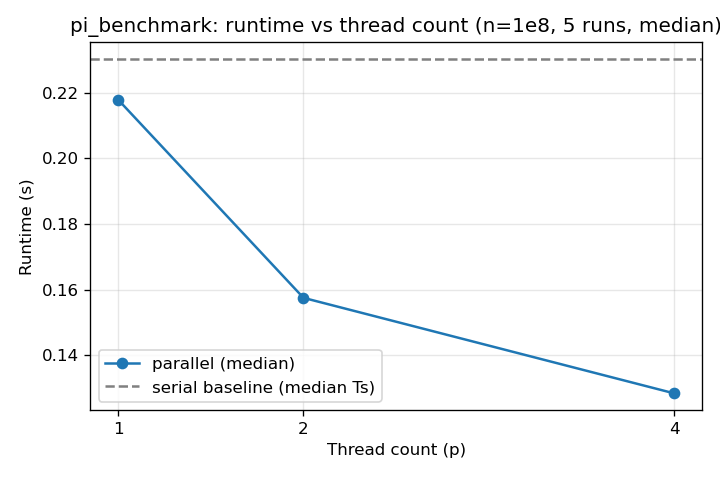
\includegraphics[width=0.85\textwidth]{pi_runtime.png}
\caption{Runtime median vs jumlah thread ($n=10^8$); garis putus-putus = baseline serial.}
\end{figure}

\begin{figure}[htbp]\centering
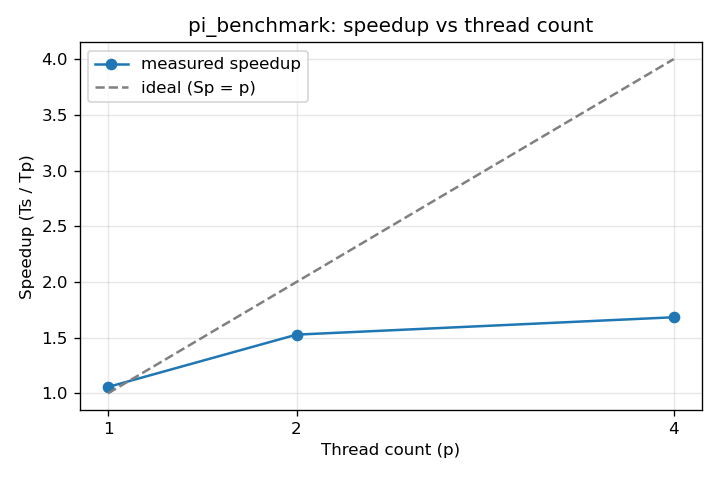
\includegraphics[width=0.85\textwidth]{pi_speedup.png}
\caption{Speedup terukur vs jumlah thread; garis putus-putus = speedup ideal $S_p=p$.}
\end{figure}

\subsection{Validasi numerik}
Selisih serial--paralel maksimum $7{,}438\times10^{-13} < 10^{-8}$ (lolos,
\texttt{exit=0} pada seluruh 15 run); \texttt{reference\_error} maksimum
$6{,}333\times10^{-13}$ terhadap \texttt{acos(-1)}. Kedua implementasi
cocok dan akurat.

\subsection{Penjelasan skala dan jawaban pertanyaan akhir}
\begin{enumerate}
\item Tercepat pada 4 thread ($S_p=1{,}68$), tetapi efisiensinya hanya 0,42:
4 thread pada 2 vCPU adalah oversubscription. Skala ``jujur'' terlihat pada
2 thread: $S_p=1{,}53$, $E_p=0{,}76$.
\item Satu thread OpenMP (0,218 s) tidak persis sama dengan loop serial
(0,230 s): region OpenMP satu thread tetap menanggung overhead pembentukan
tim dan reduction, walau di sini warm-up membuatnya sedikit lebih cepat ---
keduanya baseline yang berbeda dan tidak dapat dipertukarkan.
\item Memperbesar ukuran masalah membuat paralelisme lebih berguna: overhead
tetap (pembentukan tim, sinkronisasi) teramortisasi oleh porsi kerja paralel
yang lebih besar.
\item {\sloppy Pengukuran tambahan yang membantu menjelaskan perlambatan: pinning
thread (\cmd{OMP\_PROC\_BIND}), waktu per thread, bandwidth memori,
frekuensi CPU selama run, dan variasi urutan run untuk mendeteksi interferensi VM.\par}
\end{enumerate}
Batas Amdahl $S_p \le 1/(f + (1-f)/p)$ adalah batas ideal dengan kerja tetap;
program riil juga menghadapi batas bandwidth memori, ketidakseimbangan beban,
dan interferensi VM --- thread lebih banyak tidak harus berarti lebih cepat.

\section{Mini-project: Perkalian matriks paralel}
\label{sec:matmul}
Berkas: \texttt{src/matmul.c} mengimplementasikan $C=AB$ untuk matriks
$N\times N$ padat dalam array 1D row-major, alokasi heap, dalam tiga varian:
serial, \cmd{\#pragma omp parallel for schedule(static)} pada loop $i$,
dan varian \cmd{collapse(2)} pada loop $i,j$. Akumulasi memakai variabel
lokal per iterasi sehingga tidak perlu reduction antar thread.

\evidence{shot_10_matmul.png}{Verifikasi $n=256$, 2 thread: cek identitas tepat, paralel identik dengan serial, speedup 2,00.}

Hasil ($n=256$, waktu hanya perkalian):
\begin{center}
\begin{tabularx}{\textwidth}{rcccc}
\toprule
Thread & Serial (s) & Paralel (s) & Collapse(2) (s) & Speedup par./coll. \\
\midrule
1 & 0,0488 & 0,0698 & 0,0428 & 0,70 / 1,14 \\
2 & 0,0435 & 0,0217 & 0,0263 & 2,00 / 1,65 \\
4 & 0,0422 & 0,0233 & 0,0214 & 1,81 / 1,98 \\
\bottomrule
\end{tabularx}
\end{center}

\begin{enumerate}
\item Cek identitas ($B=I$): $C=A$ tepat (\texttt{0.000e+00}) untuk serial
maupun paralel.
\item Nilai nontrivial deterministik: paralel dan collapse(2) identik dengan
serial (\texttt{0.000e+00} $<$ toleransi $10^{-9}$) pada seluruh konfigurasi.
\item \cmd{collapse(2)} mendistribusikan ruang iterasi gabungan $(i,j)$;
setiap keluaran tetap memiliki akumulator lokalnya sendiri. Pada $n=256$,
collapse(2) sedikit lebih baik pada 4 thread (1,98 vs 1,81) karena
pembagian kerja lebih halus.
\item $n=128$ terlalu kecil ($\approx$3 ms) sehingga hasilnya didominasi
noise --- pembanding tetap memakai baseline serial yang setara (urutan loop
dan flag identik), sesuai prinsip tutorial.
\end{enumerate}

\section{Refleksi: satu bug dan diagnosisnya}
\label{sec:reflect}
Bug yang ditemui: program mini-project \texttt{matmul.c} gagal dikompilasi
dengan galat
\begin{lstlisting}
src/matmul.c:107:50: error: expected '#pragma omp' clause before '{' token
\end{lstlisting}
pada baris \cmd{\#pragma omp parallel default(none) shared(n) \{ (void)n; \}}.
Diagnosis dilakukan dengan program uji minimal: pragma yang diikuti blok
\cmd{\{} pada \emph{baris berikutnya} dikompilasi dengan baik, sedangkan
\cmd{\{} pada \emph{baris yang sama} dengan pragma selalu gagal. Ternyata
parser OpenMP GCC tidak menerima kurung kurawal blok terstruktur pada baris
yang sama dengan direktif \cmd{\#pragma omp parallel} --- blok terstruktur
harus menjadi unit sintaksis tersendiri setelah direktif. Perbaikan: pindahkan
\cmd{\{} ke baris berikutnya; kompilasi kemudian bersih tanpa warning. Bug
ini tidak terkait semantik paralelisme sama sekali, melainkan aturan
penulisan direktif --- pengingat bahwa pesan galat kompiler OpenMP perlu
dibaca harfiah per baris.

\section{Reproduksi}
\label{sec:repro}
Seluruh sumber, Makefile, bukti output mentah (\texttt{evidence/}),
screenshot, dan plot tersedia pada repositori:
\url{https://github.com/aufaakmalbunaya/openmp-tutorial}.
Perintah reproduksi persis:
\begin{lstlisting}
make
export OMP_DYNAMIC=FALSE
OMP_NUM_THREADS=4 ./bin/hello_openmp
OMP_NUM_THREADS=4 ./bin/data_sharing
for t in 1 2 4; do OMP_NUM_THREADS=$t ./bin/vector_add; done
OMP_NUM_THREADS=4 ./bin/sum_methods
for s in static "static,1" "dynamic,1" "guided,1"; do \
  OMP_NUM_THREADS=4 OMP_SCHEDULE="$s" ./bin/schedules; done
OMP_NUM_THREADS=4 ./bin/phases
OMP_NUM_THREADS=4 ./bin/tasks
for t in 1 2 4; do OMP_NUM_THREADS=$t ./bin/pi_benchmark; done
OMP_NUM_THREADS=2 ./bin/matmul 256
\end{lstlisting}
Laporan ini dikompilasi dari \texttt{latex\_report/laporan\_openmp.tex}
dengan pdfLaTeX (dua pass).

\section*{Referensi}
Tutorial ``OpenMP Programming'' (22 halaman, edisi bahasa Inggris) beserta
dokumentasi GCC OpenMP dan spesifikasi OpenMP 5.1/5.2 yang dirujuk di
dalamnya.

\end{document}
